
% \usepackage[linesnumbered,vlined]{algorithm2e}


\section{Objetivo}

Conocer el funcionamiento de la unidad elemental con la cual se construyen las redes neuronales: el perceptrón, y lograr implementar un perceptrón simple que aprenda las operaciones \classname{AND} y \classname{OR} para tres variables.

\begin{auxcode}
 \caption{Perceptrón}
 \centering
 \hurl{\auxprefix ia-perceptron}
\end{auxcode}

\section{Introducci\'on}

\quotes{Una red neuronal se puede definir como un modelo de razonamiento basado en el cerebro humano} \parencite[166]{Nengnevitsky2005}. Basándonos en el libro de Negnevisky explicaremos cómo funciona el cerebro, cómo las Redes Neuronales modelan el cerebro, cómo aprenden y finalizaremos con el Perceptrón \parencite[cap. 6]{Nengnevitsky2005}.


\subsection{Redes Neuronales Artificiales}

Sabemos que el cerebro consiste en un conjunto densamente interconectado de unidades básicas de procesamiento, llamadas neuronas. El cerebro humano contiene cerca de 86 mil millones de neuronas \parencite{Herculano-Houzel2009} y entre 100 y 500 billones de conexiones \parencite{Drachman2005}, llamadas \textbf{sinapsis}.\par

A pesar de que cada neurona tiene una estructura muy simple, un conjunto (aunque sea pequeño) de estos elementos constituye un poder de procesamiento enorme. Una neurona está constituida por un cuerpo celular, llamado \textbf{soma}, un conjunto de fibras llamadas \textbf{dendritas}, y una única fibra larga llamada \textbf{axón}. La figura~\ref{fig:P9screen1} representa dos neuronas conectadas.

Las señales se propagan de una neurona a otra por medio de reacciones electroquímicas complejas. Las substancias químicas que se liberan desde las sinapsis causan un cambio en el potencial eléctrico del cuerpo celular de la neurona. Cuando este potencial sobrepasa su umbral, una señal eléctrica, llamada \textbf{potencial de acción}, se manda a través del axón. Este pulso se dispersa y eventualmente llega a las sinapsis, haciendo que estas incrementen o decrementen su potencial. Pero el descubrimiento más interesante es que las neuronas exhiben \textbf{plasticidad}.\par

Esta plasticidad permite que las conexiones hacia las neuronas que conducen a la \quotes{respuesta correcta} se vean fortalecidas, mientras que las conexiones que llevan a la \quotes{respuesta equivocada} sean debilitadas. Como resultado, las redes neuronales tienen la habilidad de aprender mediante la experiencia.

\begin{figure}
  \centering
  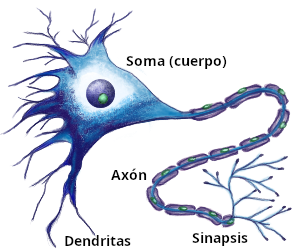
\includegraphics[width=0.5\textwidth]{perceptron/NeuronaPartes.png}
  \caption{Partes de una neurona biológica. \textbf{Autor:} Arriola Ríos}
  \label{fig:P9screen1}
\end{figure}

\subsubsection{Redes neuronales}

El cerebro humano adquiere su gran capacidad de cómputo de la interconexión de millones de neuronas, especializadas para cubrir diferentes funciones como visión, tacto, procesamiento de información abstracta, etc. y organizadas en macroestructuras que aún se estudian hoy en día \parencite{Mesulam1998}.  Por ello, una red neuronal artificial se conforma por numerosos perceptrones que se conectan entre sí usando conexiones con un peso dado, pasando señales de una neurona a otra. Cada neurona recibe un número de señales de entrada a través de sus conexiones, pero sólo produce una salida, como se muestra en la figura~\ref{fig:P9screen2}. Esta señal de salida se transmite por la conexión saliente de la neurona (lo equivalente al axón en la neurona biológica). Esta conexión saliente, a su vez, se separa en varias ramas que transmiten la misma señal. Estas ramas terminan como conexiones de entrada de otras neuronas en la red.

\subsubsection{Aprendizaje}

\noindent Las neuronas se conectan mediante enlaces que tienen un peso asociado a ellos. Estos pesos son los medios para guardar información a largo plazo. Expresan la importancia de cada entrada de la neurona. Entonces, las redes neuronales \quotes{aprenden} por medio de ajustes a estos pesos.


\subsection{Neuronas Artificiales}

\begin{figure}[ht]
  \centering
  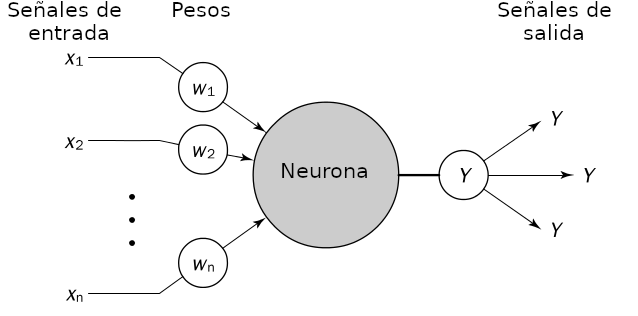
\includegraphics[scale=0.35]{perceptron/screen2.png}
  \caption{Diagrama de un perceptrón. \parencite[168]{Nengnevitsky2005}}
  \label{fig:P9screen2}
\end{figure}

\subsubsection{Cálculo de la salida}

\noindent La neurona calcula la suma de las señales de entrada multiplicadas por el peso de su conexión con la neurona siguiente (combinación lineal) y compara este resultado con un umbral $\theta$. Si el total es menor que el umbral, la salida de la neurona es (\ -1)\ , si es mayor entonces la neurona se activa y su salida es (\ 1)\ . A lo descrito anteriormente se le llama función de activación.


\subsection{Perceptr\'on}

Un perceptrón es la forma más simple de una red neuronal, ya que representa a una sola neurona.

El perceptrón consiste en un combinador lineal seguido de una función de activación. Se le aplica la función umbral a la suma con pesos de las entradas menos el umbral, la cual produce una salida positiva si la suma es positiva, o una salida negativa si la suma es negativa. El objetivo del perceptrón es clasificar entradas en una de dos clases. Esto se expresa con la siguiente función: 

\[Y = f\left(\sum_{i=1}^{n}x_iw_i-\theta\right)\]
\parencite[169]{Nengnevitsky2005}

La función escalón (\textit{sign function}) es una opción básica que puede fungir como función de activación:
\begin{align*}
 f &= \begin{cases}
       1 & \text{si } X \geq 0 \\
       0 & \text{si } X < 0
      \end{cases}
\end{align*}

\subsubsection{Aprendizaje para clasificación}

Esto se logra haciendo pequeñas modificaciones a los pesos de las entradas para reducir las diferencias entre la salida obtenida y la salida deseada. El proceso de actualización de pesos es bastante simple. Como queremos obtener (o aproximarnos a) una salida deseada, tenemos que iterar sobre un conjunto de entrenamiento (de tamaño $m$) las veces necesarias, modificando los pesos de las conexiones, hasta minimizar el error en la salida. Si para el ejemplar de entrenamiento $j$, la salida es $Y(j)$ y la salida deseada es $Y_d(j)$, entonces la función de error está dada por:

\[ e(j) = Y_d(j)-Y(j)\]
\parencite[171]{Nengnevitsky2005}

Si $e(j)$ es positivo, se necesita incrementar $Y(j)$, pero si es negativo, se necesita disminuirlo. Tomando en cuenta que cada entrada contribuye \(x_i(j) \times w_i(j)\) a la entrada total $X(j)$, nos damos cuenta que si el valor de entrada $x_i(j)$ es positivo, aumentar su peso $w_i(j)$ incrementa la salida del perceptrón, mientras que si $x_i(j)$ es negativa, un aumento en su peso $w_i(j)$ disminuye el valor de salida del perceptrón. Por lo tanto se puede establecer la siguiente regla de aprendizaje:

\[w_i(j+1) = w_i(j) + \alpha \times x_i(j) \times e(j) \]
\parencite[171]{Nengnevitsky2005}

\noindent donde $\alpha$ es la \textbf{taza de aprendizaje}, una variable no negativa menor a $1$.

\subsection{Resumen del algoritmo de aprendizaje}

\noindent En pocas palabras, se necesitan cuatro pasos para que un perceptrón aprenda a clasificar las entradas \parencite[172]{Nengnevitsky2005}:\par

\begin{enumerate}
  \item \textbf{Inicialización:} Fijar los pesos iniciales \(w_1, w_2, ..., w_n\) y el umbral $\theta$ a números aleatorios en el rango $[-0.5, 0.5]$ (recomendado).
  
  \item \textbf{Activación:} Para un ejemplar $j$, activar el perceptrón aplicando las entradas\\ \(x_1(j), x_2(j), ..., x_n(j)\).
  \[Y(j) = f\left(\sum_{i=1}^{n}x_i(j)w_i(j)-\theta\right)\]
  donde $n$ es el número de entradas y $f$ es la función de activación.
  
  \item \textbf{Entrenamiento de pesos:} Se actualizan los pesos del perceptrón:
  \[w_i(t+1)=w_i(t)+\Delta w_i(t)\]
  donde \(\Delta w_i(t)\) es la corrección del peso al tiempo $t$ para el ejemplar $j$, que se calcula de la siguiente forma:
  \[\Delta w_i(t)=\alpha \times x_i(j) \times e(j)\]
  
  El umbral $\theta$ se queda fijo en el valor que le fue asignado al inicio.
  
  \item \textbf{Iteración:} Repetir los pasos 2 y 3 para cada ejemplar del conjunto de entrenamiento hasta minimizar lo mejor posible el error. Si el resultado no es satisfactorio, continuar ejecutando otra vez desde el primer ejemplar.
  \label{algo:b}
\end{enumerate}

\section{Desarrollo e implementaci\'on}

\noindent Deberán crear dos perceptrones, uno que aprenda la operación \classname{AND} y otro la operación \classname{OR}, ambas de tres variables. Cada neurona tendrá cuatro entradas, tres para las entradas de la operación lógica y una para el sesgo $\theta$.\par

\begin{figure}[H]
    \centering
    \begin{subfigure}[b]{0.4\textwidth}
        \centering
        \begin{tabular}{ l l c | r }
          $x_1$ & $x_2$ & $x_3$ & $Salida$\\ \hline
          0 & 0 & 0 & 0  \\ \hline
          0 & 0 & 1 & 0  \\ \hline
          0 & 1 & 0 & 0  \\ \hline
          0 & 1 & 1 & 0  \\ \hline
          1 & 0 & 0 & 0  \\ \hline
          1 & 0 & 1 & 0  \\ \hline
          1 & 1 & 0 & 0  \\ \hline
          1 & 1 & 1 & 1  \\
        \end{tabular}
        \caption{Operación AND}
    \end{subfigure}
    ~ 
    \begin{subfigure}[b]{0.4\textwidth}
        \centering
        \begin{tabular}{ l l c | r }
          $x_1$ & $x_2$ & $x_3$ & $Salida$\\ \hline
          0 & 0 & 0 & 0  \\ \hline
          0 & 0 & 1 & 1  \\ \hline
          0 & 1 & 0 & 1  \\ \hline
          0 & 1 & 1 & 1  \\ \hline
          1 & 0 & 0 & 1  \\ \hline
          1 & 0 & 1 & 1  \\ \hline
          1 & 1 & 0 & 1  \\ \hline
          1 & 1 & 1 & 1  \\
        \end{tabular}
        \caption{Operación OR}
    \end{subfigure}
\end{figure}

Su aplicación deberá permitir elegir distintos conjuntos de entrenamiento, en particular, tienen que especificar al menos 5 conjuntos de entrenamiento : 

\begin{enumerate}
  \item \texttt{[[0,0,0,0],[1,1,1,1]]} para AND y OR
  \item El conjunto que contenga todas las combinaciones posibles de entradas
  \item Y tres conjuntos más con elementos distintos, tomados de las tablas mostradas anteriormente.
\end{enumerate}

Con el formato: \[\texttt{[}x_1, x_2, x_3, Salida\texttt{]} \]

\noindent Esto para que se den una idea ustedes de lo importante que son los conjuntos de entrenamiento de un perceptrón.
También tienen que mostrar el proceso de entrenamiento, y una vez entrenado el perceptrón, debe permitir hacer consultas de estas operaciones lógicas.\par
Para probar su perceptrón, deberán utilizar el siguiente conjunto de entradas:

\[\texttt{[}\texttt{[}0,0,0\texttt{]}, \texttt{[}1,0,1\texttt{]}, \texttt{[}0,0,1\texttt{]}, \texttt{[}1,1,1\texttt{]} \texttt{]}\]

Observen que el éxito al entrenar el perceptrón dependerá fuertemente de los datos que quedaron en su conjunto de entrenamiento.



\section{Requisitos y resultados}

Entreguen el código donde implementaron el perceptrón y su entrenamiento.  Generen un reporte con observaciones de cómo se comporta el perceptrón con cada uno de los conjuntos de entrenamiento. Lo podrán programar en \classname{Java} o \classname{Python}. No olviden comentar su código.\medskip


% \begin{thebibliography}{1}

  % \bibitem{notes} Michael Nengnevitsky {\em Artificial Intelligence: A guide to Intelligent Systems}, 2005 :
  % Pearson Education Limited, Essex, England .

% \end{thebibliography}

